\subsection{Project Overview}\label{subsec:project-overview}
The focus of my research project was on developing a model for multi-modal traffic prediction, specifically targeting
cars and wheelchairs.
This project aimed to address the unique challenges faced by mobility-impaired individuals, particularly those using
wheelchairs, by providing traffic predictions that consider their specific needs.
While existing platforms like Google Maps and Apple Maps offer itinerary recommendations, they often fall short when it
comes to detailed traffic predictions for wheelchair users.
Additionally, concerns over data privacy with these large platforms underscore the need for an open-source alternative.

The importance of this project lies in its potential to fill a gap in current traffic prediction systems by including
modes of transportation that are often overlooked, such as wheelchairs.
Unlike traditional itinerary recommendation systems, this project focuses on predicting traffic patterns rather than
suggesting routes, which adds an extra layer of complexity and utility.

To solve this problem, the project involved adapting the Diffusion Convolutional Recurrent Neural Network (DCRNN) model
to handle the complexity of multi-modal traffic prediction.
The model was upgraded to consider both cars and wheelchairs, with a specific focus on capturing the spatial and
temporal dependencies in traffic data.
Additionally, a method was developed to derive wheelchair traffic data from the METR-LA dataset, which contains only car
traffic data.

The ultimate goal of the project was to produce a model capable of delivering accurate traffic predictions for both cars
and wheelchairs, thereby contributing to a more inclusive and comprehensive traffic prediction system.

\subsection{Objectives and Goals}\label{subsec:objectives-and-goals}
The primary goal of this project was to develop a model capable of performing accurate multi-modal traffic predictions
for both cars and wheelchairs.
While there were no strict performance targets set for the model, the project aimed to achieve a level of accuracy that
would be competitive with existing models in the field.
To evaluate the model's performance, we used Mean Absolute Error (MAE) and Root Mean Square Error (RMSE) as loss
metrics, comparing these results against those of other established models.

In addition to the technical objectives, I also had several personal goals for this project.
These included deepening my understanding of the research process and methodology, expanding my knowledge of machine
learning, and improving my skills in Python programming and LaTeX for academic writing.
These personal objectives were crucial for my professional development and aligned with my broader career aspirations in
the field of artificial intelligence and research.

\subsection{Scope of Work}\label{subsec:scope-of-work}
The development of the multi-modal traffic prediction model involved several key tasks and activities.
The first step was obtaining and understanding the METR-LA dataset, which provided the foundational data for car
traffic.
Given the absence of publicly available datasets for wheelchair traffic, a significant portion of the project involved
developing a method to derive wheelchair data from the existing car traffic data.

The next phase was designing a new architecture for the model, which required considerable effort in debugging and
refining the model to ensure it could effectively handle the complexities of multi-modal traffic prediction.
Training the model was another crucial task, which I accomplished using Kaggle's computational resources.
Although these resources were limited for working with Graph Neural Networks, they were sufficient to complete
the project.

The main deliverables of the project include the research paper, which documents the methodology, data derivation
process, model architecture, and results.
Additionally, the newly created dataset, which integrates car and wheelchair traffic data, is another important output
of the project.
While the model itself was not saved due to its suboptimal performance, the insights and methodologies developed during
the project remain valuable contributions.

\subsection{Methodology and Approach}\label{subsec:methodology-and-approach}

\subsubsection{Overall Approach and Strategy}\label{subsubsec:overall-approach-and-strategy}
The project aimed to adapt an existing model, the Diffusion Convolutional Recurrent Neural Network (DCRNN), to handle
the complexities of multi-modal traffic prediction, specifically for cars and wheelchairs.
The overall approach involved several key stages: understanding and processing the existing METR-LA dataset, deriving
wheelchair traffic data,adapting the model architecture to accommodate multiple modes of transportation, and training
the model to predict traffic patterns.

\subsubsection{Key Methods and Techniques}\label{subsubsec:key-methods-and-techniques}
\begin{enumerate}
    \item \textbf{Model Adaptation}:
    \begin{itemize}
        \item
        The DCRNN model was adapted to consider both cars and wheelchairs by introducing a custom diffusion convolution
        operation to capture spatial dependencies in traffic data.
        Temporal dependencies were managed using Gated Recurrent Units (GRU), modified with the custom diffusion
        convolution to create a Diffusion Convolution Gated Recurrent Unit (DCGRU).
        \item
        The model's architecture retained the original encoder-decoder structure of the DCRNN but included key
        modifications.
        A new convolution operation, inherited from the PyTorch Geometric library's MessagePassing class, was used to
        enhance spatial dependency capture.
        Additionally, a multi-headed attention mechanism was added to allow the model to differentiate between the
        various locomotion modes.
    \end{itemize}

    \item \textbf{Data Derivation}:
    \begin{itemize}
        \item
        Due to the lack of available wheelchair traffic data, a new method was developed to derive this data from the
        car traffic data in the METR-LA dataset.
        The process involved calculating an accessibility score using OpenStreetMap data, which was then applied to
        adjust the car traffic speeds to reflect wheelchair speeds.
        The final wheelchair traffic data was generated by scaling and introducing noise to simulate real-world
        variability.
    \end{itemize}

    \item \textbf{Training and Evaluation}:
    \begin{itemize}
        \item
        The model was implemented using PyTorch and associated libraries, with training conducted on the Kaggle
        platform.
        The dataset was split into training, validation, and test sets, with inputs shaped to capture various features,
        including speed, time of day, day of the week, and locomotion mode.
        \item
        Model performance was evaluated using Mean Absolute Error (MAE) and Root Mean Square Error (RMSE)
        metrics,comparing results against baseline models.
        The evaluation revealed that while the model performed well for individual modes (cars or wheelchairs), its
        performance on combined multi-modal predictions was less satisfactory, highlighting the complexity of the task.
    \end{itemize}
\end{enumerate}

\subsubsection{Challenges and Solutions}\label{subsubsec:challenges-and-solutions}
One of the main challenges was the derivation of wheelchair traffic data, as no pre-existing datasets were available.
The innovative method developed to generate this data introduced potential biases, but it was a necessary step given the
time, resources and data constraints we had.
Another challenge was the model's scalability and generalization, as its performance varied significantly across
different transportation modes.
While the model showed promising results, further improvements in architecture and data collection are necessary for better
scalability and generalization.

\subsection{Project Timeline}\label{subsec:project-timeline}
\begin{figure*}[htbp]
    \centering
    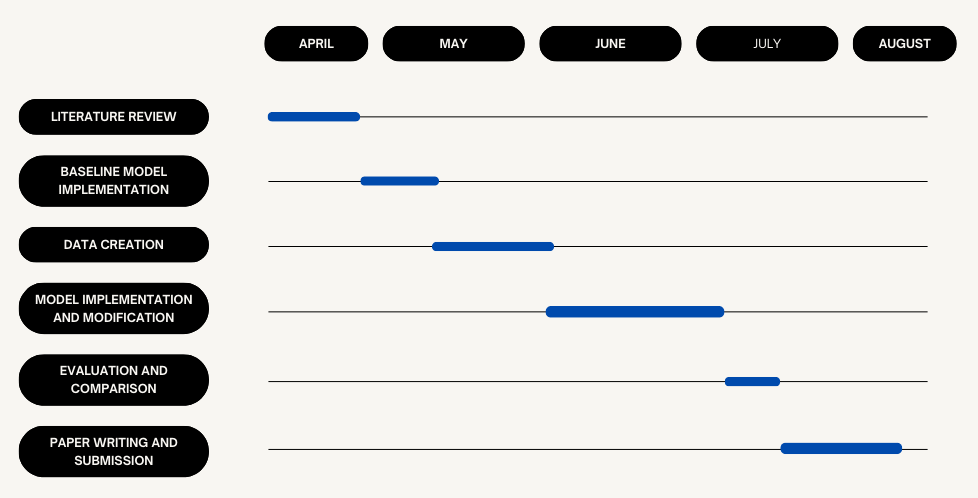
\includegraphics[width=1\textwidth]{images/gantt}
    \caption{
        Gantt diagram showing the project timeline and key milestones.
    }
    \label{fig:model}
\end{figure*}

\subsection{Outcomes and Results}\label{subsec:outcomes-and-results}
The project adapted the DCRNN model for multi-modal traffic prediction, focusing on cars and wheelchairs.
A key outcome was developing a method to derive wheelchair traffic data from existing car traffic data, addressing the
lack of wheelchair-specific datasets.
The model performed well for car traffic predictions, but its multi-modal predictions had higher error rates,
highlighting the complexity of the task.
Despite this, the project introduced valuable methodologies and laid the groundwork for future improvements in
wheelchair traffic prediction.